\documentclass{beamer} 
\usepackage{graphicx}
\usepackage[compatibility=false]{caption}
\usepackage{subcaption}

% Coloca os conteúdos auto-gerados, como "Figura", em português
%\usepackage[portuguese]{babel}

% Aceita caracteres UTF-8 no arquivo fonte
\usepackage[utf8]{inputenc}

% Ajuda a hifenização de palavras com acento
\usepackage[T1]{fontenc}

% Permite deixar uma imagem sobre outra.
\usepackage{stackengine}

\DeclareMathOperator*{\argmax}{arg\,max}

% Define the name of the game
\newcommand{\rawgamename}{Sweet Switches}
\newcommand{\itgamename}{\emph{\rawgamename}}
\newcommand{\gamename}{\textbf{\emph{\rawgamename}}}
\usepackage{url}

\usetheme{Boadilla}
\usecolortheme{whale}

\def\beamertemplatetransparentcoveredmedium{\setbeamercovered{transparent=40}}
\beamertemplatetransparentcoveredmedium

\makeatletter
\setbeamertemplate{footline}{%
    \leavevmode%
    \hbox{%
        \begin{beamercolorbox}[wd=0.26\paperwidth,ht=2.25ex,dp=1ex,center]%
                              {title in head/foot}%
            \usebeamerfont{title in head/foot}\insertshorttitle%
        \end{beamercolorbox}%
        \begin{beamercolorbox}[wd=0.68\paperwidth,ht=2.25ex,dp=1ex,center]%
                              {author in head/foot}%
            \usebeamerfont{author in head/foot}\insertshortauthor%
        \end{beamercolorbox}%
        \begin{beamercolorbox}[wd=0.06\paperwidth,ht=2.25ex,dp=1ex,center]%
                              {author in head/foot}%
            \insertframenumber{}/\inserttotalframenumber%
        \end{beamercolorbox}%
    }%
    \vskip0pt%
}
\makeatother


%%%%%%%%%%%%%%%%%%%%%%%%%%%%%%%%%%%%%%%%%%%%%%%%%%%%%%%%%%%%%%%%%%%%%
% TODO: Make the first page be the similar to MenuState of the game %
%%%%%%%%%%%%%%%%%%%%%%%%%%%%%%%%%%%%%%%%%%%%%%%%%%%%%%%%%%%%%%%%%%%%%

% DRAFT%
% * Introducing programming concepts without forcing code writing is a goal of
%   \gamename

% * Make a presentation start with a story

% # STORY (main scenario of use of SS):
%   Imagine that a class of students is presented to SS. After the students try
%   solving the puzzles, the teacher can help them to make a deliberation about
%   each solution.

%   At this moment, the teacher could expose the puzzles as a logic challenges
%   and explain:
%   \item Possible alternative solutions
%   \item Common mistakes

%   After solving a group of SS puzzles, the teacher could start the
%   introduction of computing concepts in the traditional way (or ``formal''
%   way).

%   But then he/she will be able to describe most those concepts using examples
%   based on ``conveyors'' and ''devices''.

%   Finally the teacher could solve SS puzzles again explaining them in terms
%   of execution flow and programming statements.

%   This way we expect to increase students engagement and reduce the learning
%   barrier of this subject.

% # MOTIVATION 1:
%   Been class assistants of \emph{Introduction to Computing}, the main
%   difference we have noted from \textbf{Computer Science} students to the
%   others was that the formers already have a ''procedural way of thinking''
%   when they arrive at the corse. By the other hand, most of other students
%   haven't developed that mindset previously and, as consequence, face a
%   grate challenge when are introduced to a programming language.

%   With SS we want to help students to develop that mindset much before
%   college. Ideally when they are still kids.

%   = Why do we want to make every student (or kid) to understand the basics
%     of computer programming? =

%   * Do we want to conquer the world with an army of programmers? *
%   Yes!

%   But besides that, the thruth is that today's world is rulled by softwares
%   and computers, and it is essential to understand the basics about them in
%   order to live surounded by all this technology.

%   A great way to describe that necessity is found in a report prepared for
%   the UK Computing Research Committee\footnote{Computing
%   at School: the state of the nation, 2009}:
%     
%   \emph{if on one hand
%     learning how to use computers can be seen as to learning how to
%     read, on the other hand learning how to program is similar to
%     learning how to write. They are both skills that everyone should have,
%     even
%     though a minority will become professionals (writers or programmers).
%   }

% # MOTIVATION 2:
%   The study of computer programming elements at primary school is
%   increasingly being acknowledged as equally important as other disciplines
%   such as math or science.

%   The main reason for that is that the skills required for programming
%   computers are definitely valuable for education, since they involve
%   procedural thinking, problem solving through trial and error, creativity,
%   thinking about thinking, and analysis and exploration of data[6].

% # About the game itself:
% * SS is not another "program the movement" game.
%   -> Most of the usefullness of programs relies on their's capacity of ``make
%      decisions''
%   -> The format of games about programmed movimentation usually falls into
%      one of the following:
%      - They are accecible for a wide range of people, but don't provide
%        contitional structures;
%      or...
%      - They are too complex and is atractive only for programmers (AI
%        programmers actually).

% * ANALOGIES:
%   - Conveyor belt: can be seen as the execution flow of a computer program
%   - Devices: can be interpreted as operations that affect the program execution
%       (and the output)
%   - Devices with conditional behavior: are imediately recognized as branching
%       points in the execution flow.
%   - Loops are visually identified as a way of passing more then once on an
%     execution portion.




\title{\gamename}
\author[\url{http://www.ime.usp.br/~lidet/sweet-switches}]%
       {Vinícius K. Daros, Luiz C. Vieira,\\
        Adalberto B. C. Pereira, Flávio S. C. da Silva}
\institute{Laboratory of Interactivity and Digital\\
           Entertainment Technology (LIDET)\\[1em]
           University of São Paulo - Brazil}
\date{iGam4ER 2014}

\begin{document}
{
\setbeamertemplate{footline}{}
\maketitle
}
\addtocounter{framenumber}{-1}

\section{What is}
    \begin{frame}{}
        \centering
        \huge
        What is\\\itgamename?
    \end{frame}

    \begin{frame}{What is \gamename?}
        \centering
        \begin{minipage}{0.48\textwidth}
            In \itgamename\ players will face a series of puzzles inside ice
            cream factories.\\[0.5em]
            \pause

            The objective is to attach devices to conveyor belts in order to
            respond to a production request.\\[0.5em]
        \end{minipage}
        \hfill%
        \begin{minipage}{0.48\textwidth}
            \centering
            
\includegraphics[width=0.75\textwidth]{images/sweetswitches}
            \vskip 1em

            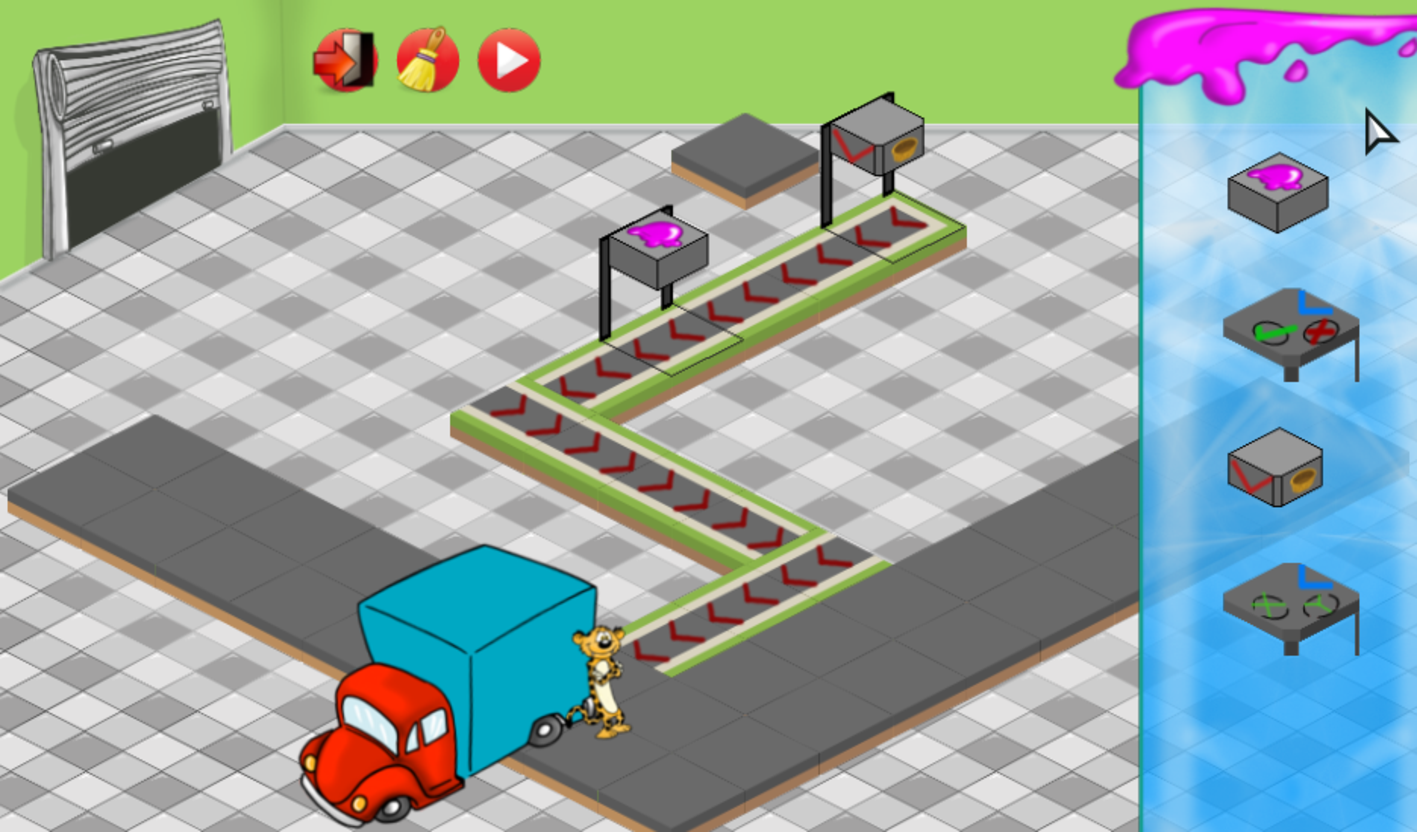
\includegraphics[width=0.9\textwidth]{images/screen1}
        \end{minipage}
    \end{frame}

\section{Objectives}
    \begin{frame}{}
        \centering
        \huge
        Project objectives
    \end{frame}

    \begin{frame}{Objectives}
        \centering
        \begin{minipage}{0.55\textwidth}
            \begin{enumerate}
                \item Be a fun puzzle game\\\vskip 1.5em

                \pause
                \item Be engaging\\\vskip 1.5em

                \pause
                \item Foster computational thinking\\(subliminally)
            \end{enumerate}
        \end{minipage}
    \end{frame}

\section{Motivations}
    \begin{frame}{}
        \centering
        \huge
        Motivations
    \end{frame}

    \begin{frame}{Motivation 1}
%The study of computer programming elements at primary school is
%increasingly being acknowledged as equally important as other disciplines
%such as math or science.
        Then importance given to computer programming elements at primary school
        is notably increasing.\\[2em]

        Skills required from programming computers are definitely valuable for
        other disciplines, since they involve\footnote{\emph{The role of
        computer programming in education}, Ken Kahn, 1999}:
        \vskip 2em

        \centering
        \begin{minipage}{0.6\textwidth}
            \begin{itemize}
                \item Procedural thinking
                \item Problem solving through trial and error
                \item Creativity
                \item Thinking about thinking
                \item Analysis and exploration of data
            \end{itemize}
        \end{minipage}

%The main reason for that is that the skills required for programming
%computers are definitely valuable for education, since they involve
%procedural thinking, problem solving through trial and error, creativity,
%thinking about thinking, and analysis and exploration of data
%\footnote{The role of computer programming in education, 1999}
    \end{frame}

    \begin{frame}{Motivation 2}
        \centering
        Report prepared for the UK Computing Research Committee%
        \footnote{\emph{Computing at School: the state of the nation}, Simon P.
        Jones, 2009}:

        \begin{minipage}{0.8\textwidth}
        \vskip 2em
        \emph{If on one hand learning how to use computers can be seen as to
            learning how to read, on the other hand learning how to program is
            similar to learning how to write.\\
            
            They are both skills that everyone should have, even though a
            minority will become professionals (writers or programmers).
        }
        \end{minipage}
    \end{frame}

\section{Application in class}
    \begin{frame}{}
        \centering
        \huge
        Application in class
    \end{frame}

    \begin{frame}{Application in class}
        \centering
        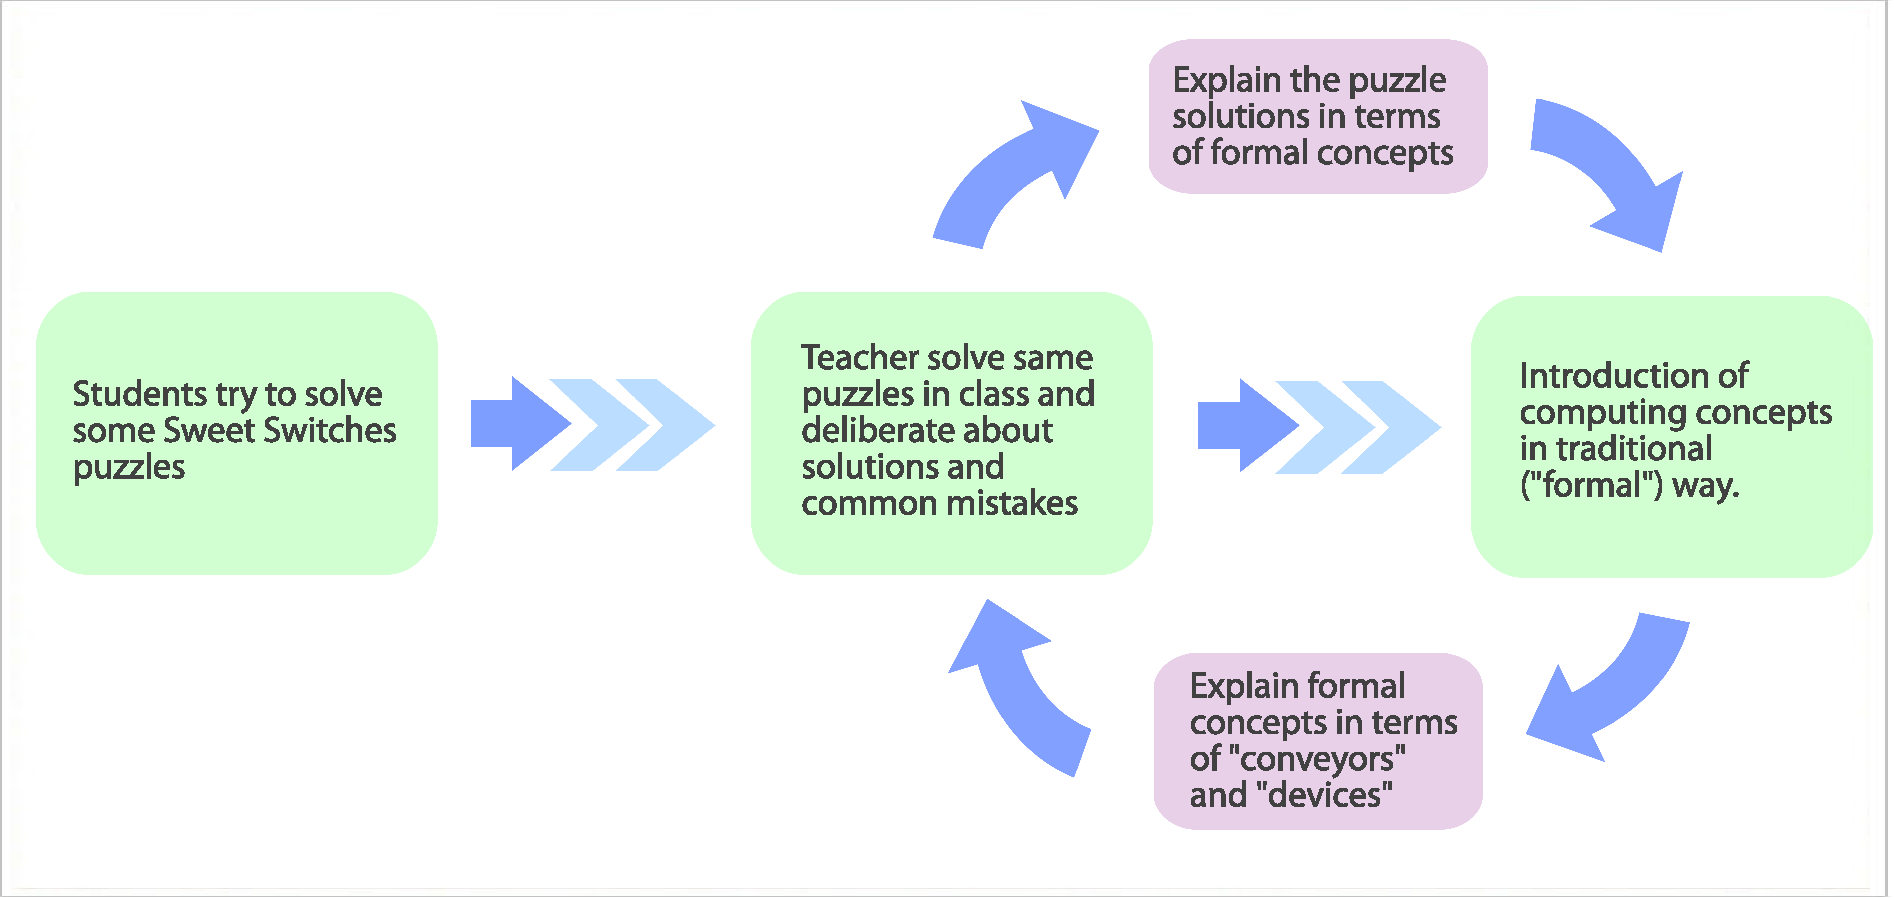
\includegraphics[width=0.9\textwidth]{images/ClassFlow}
    \end{frame}

    \begin{frame}{Game elements and analogies}
        \centering
        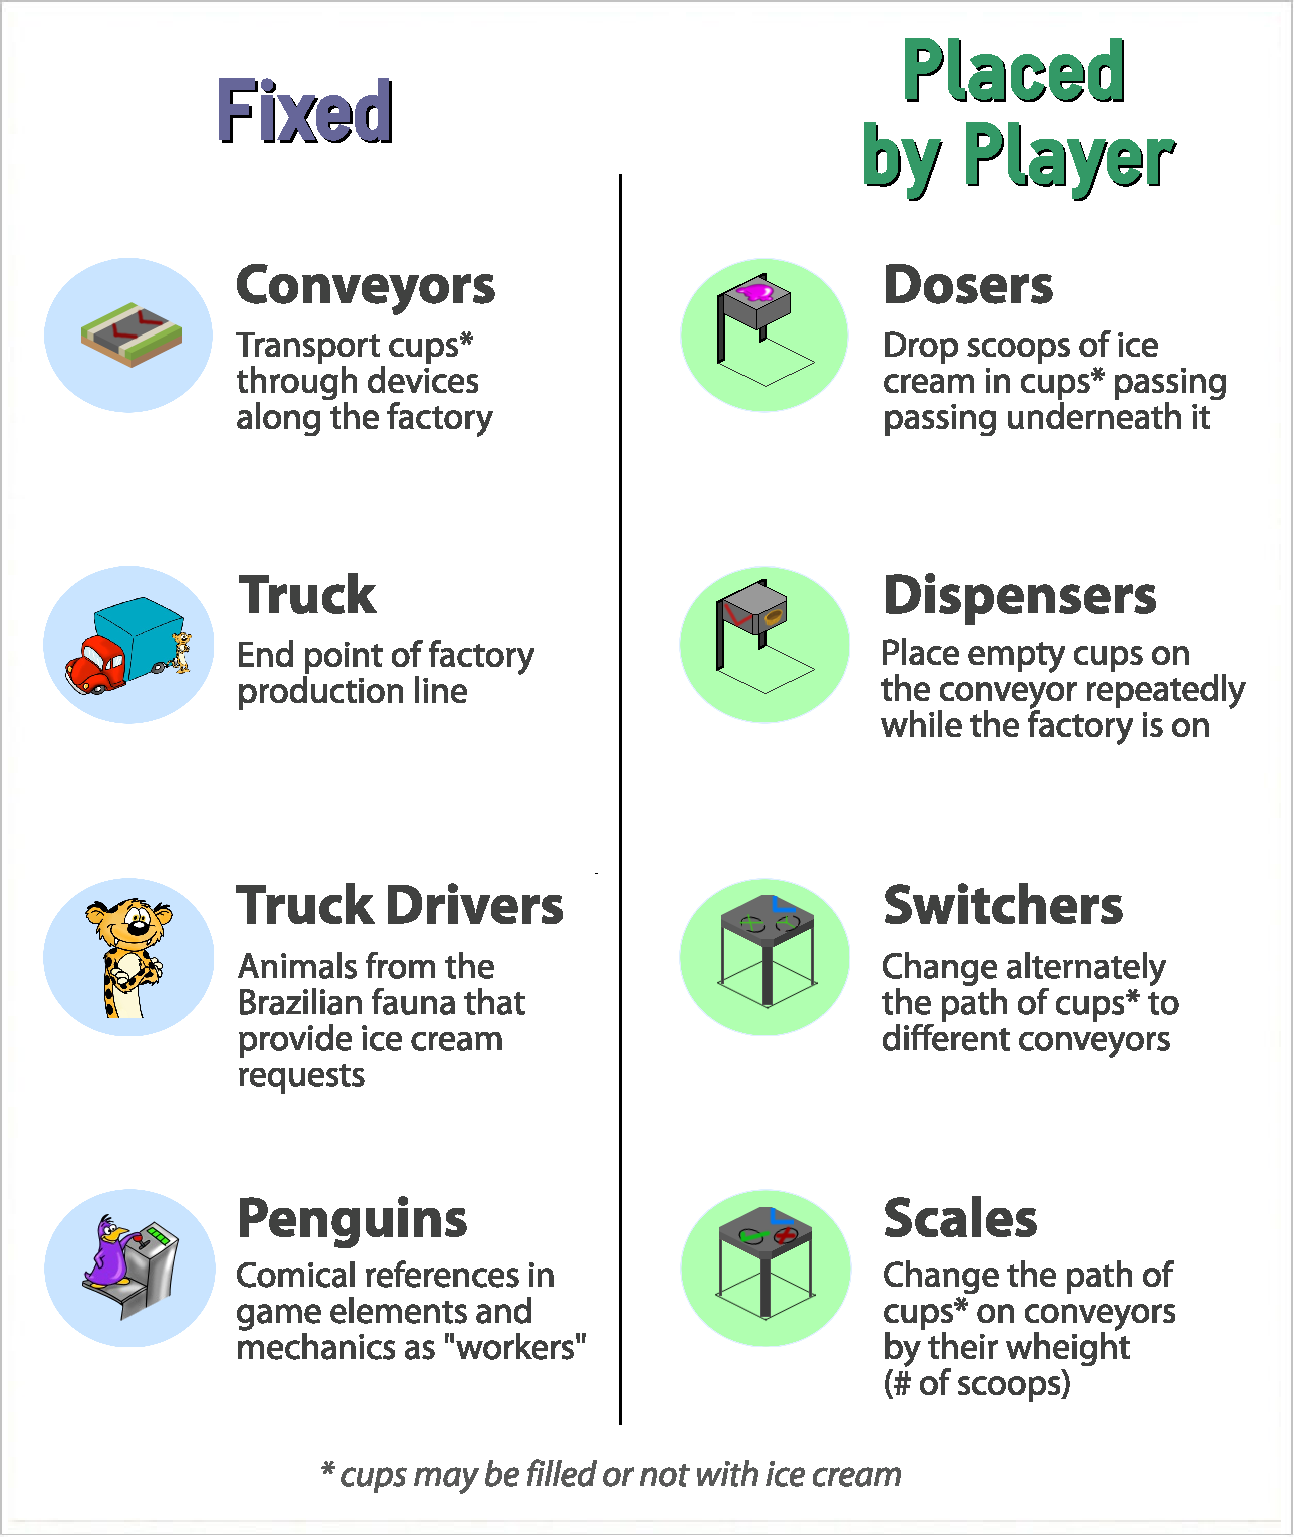
\includegraphics[height=0.9\textheight]{images/GameElements}
    \end{frame}

\section{Learning}
    \begin{frame}{}
        \centering
        \huge
        So what we expect\\players will learn?
    \end{frame}

    \begin{frame}{Direct learning}
        \centering
        By solving the puzzles in \itgamename,\\
        players will probably understand:\\[2em]

        \begin{minipage}{0.5\textwidth}
            \begin{itemize}
                \item Operation order\\[1em]
                \item Conditional execution\\[1em]
                \item Repetitions\\[1em]
                \item Debugging
            \end{itemize}
        \end{minipage}
    \end{frame}

    \begin{frame}{Tangential learning}
        \begin{center}
            Players may also learn indirectly about:
        \end{center}

        \begin{minipage}{\textwidth}
            \vskip 0.75em%
            \begin{description}[noitemsep,topsep=0pt,parsep=0pt]
                \item[Geography:]
                    Brazilian cities on the map \\[1em]
                \item[Biology:]
                    Animals of the Brazilian fauna (penguins, jaguars, macaws,
                    etc)
            \end{description}
            \vskip 0.75em%
        \end{minipage}

        \begin{minipage}{0.35\textwidth}
            \vskip -5em%
            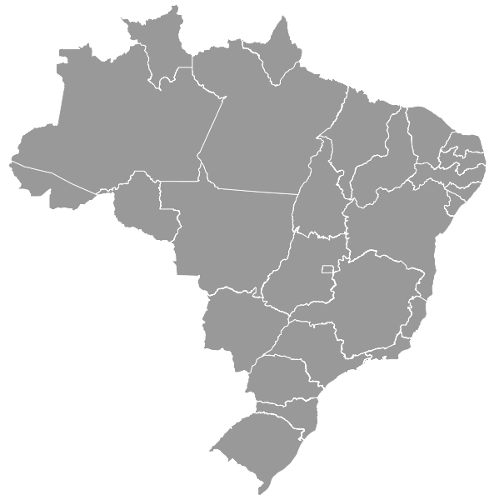
\includegraphics[width=0.9\textwidth]{images/brazil_map}
        \end{minipage}
        \hfill%
        \begin{minipage}{0.2\textwidth}
            
\includegraphics[width=0.9\textwidth]{images/onca}
        \end{minipage}
    \end{frame}
%
%\section{Demonstration}
%    \begin{frame}{}
%        \centering
%        {\huge
%        Quick game\\demonstration}
%    \end{frame}

\section{Thanks}
    \begin{frame}{Art contributors}
        Special thanks to...\\[3em]

        \centering
        \emph{Danilo Gabriel Rios}\\[1em]
        and\\[1em]
        \emph{Salvador Oliva Junior}
    \end{frame}

    \begin{frame}{}
        \centering
        {\huge
        Thank you!}
    \end{frame}
\end{document}
